\documentclass[12pt,english]{article}
\usepackage[cm]{fullpage}
\usepackage[utf8]{inputenc}
\usepackage[T1]{fontenc}
\usepackage{lmodern}
\usepackage[main=english]{babel}
\usepackage{mathtools}
\usepackage[dvipsnames]{xcolor}
\usepackage{listings}
\lstset{
	title=\texttt{\lstname},
  language=Python,
  morekeywords={assert},
  basicstyle=\footnotesize\ttfamily,
  keywordstyle=\bfseries\color{Plum},
  identifierstyle=\color{Red},
  stringstyle=\color{Green},
  commentstyle=\color{Gray},
  showstringspaces=false,
	tabsize=4,
  breaklines=true,
  prebreak=\mbox{\(\hookleftarrow\)},
  numbers=left,
  numberstyle=\footnotesize\color{darkgray},
  frame=leftline
}
\usepackage{tikz}
\usepackage[labelsep=endash]{caption}
\usepackage{hyperref}
\hypersetup{
  colorlinks=true,
	linkcolor=blue,
  urlcolor=cyan
}

\makeatletter
	\renewcommand*\and{\newline}
	\let\old@itemize\itemize%
	\renewcommand\itemize{
		\parskip=0pt
		\old@itemize%
	}
	\let\old@enditemize\enditemize%
	\renewcommand\enditemize{
		\old@enditemize%
		\parskip=\baselineskip%
	}
	\let\old@enumerate\enumerate%
	\renewcommand\enumerate{
		\parskip=0pt
		\old@enumerate%
	}
	\let\old@endenumerate\endenumerate%
	\renewcommand\endenumerate{
		\old@endenumerate%
		\parskip=\baselineskip%
	}
	\renewcommand*\@maketitle{
		\begin{titlepage}
			\begin{flushright}
				ISEP
			\end{flushright}
			\begin{center}
				\vfill
				{\Huge\@title}

				\vspace{5cm}
				{\Large\@author}

				\vfill
				{\large\@date}
			\end{center}
		\end{titlepage}
	}
	\let\old@tableofcontents\tableofcontents
	\renewcommand*\tableofcontents{
		\newpage
		\old@tableofcontents%
		\newpage
	}
	\let\old@appendix\appendix
	\renewcommand*\appendix{
		\newpage
		\old@appendix%
		{\Huge\bfseries\noindent Appendix}
	}
\makeatother

\author{
	Tanguy \textsc{Berthoud} 60989\and
	Cyprien \textsc{Bariant}\and %TODO
	Thibault \textsc{de Buisson de Courson} %TODO
}
\title{
	\textbf{PROJECT}\\
	Advanced Algorithmic and Programming
}
\begin{document}
	\maketitle
	\tableofcontents
	\parskip=\baselineskip%

	\section{Creating a graph from GTFS data}\label{sec:step:1}
	\subsection{Importing relevant GTFS data}\label{sec:step:1.1}

	Our city of choice for the project is Phoenix, in Arizona.\\
	We use the public data available here: \url{https://transitfeeds.com/p/valley-metro/68/latest}

	The difficulty here was to import the relevant data and convert it to a graph.
	Some Python libraries seem to exist but none was convenient for the project, so we needed to transform the data manually.\\
	After reading documentation on GTFS, we needed only two files from the data feed: \texttt{stops.txt} and \texttt{stop\_times.txt}.

	\begin{center}
		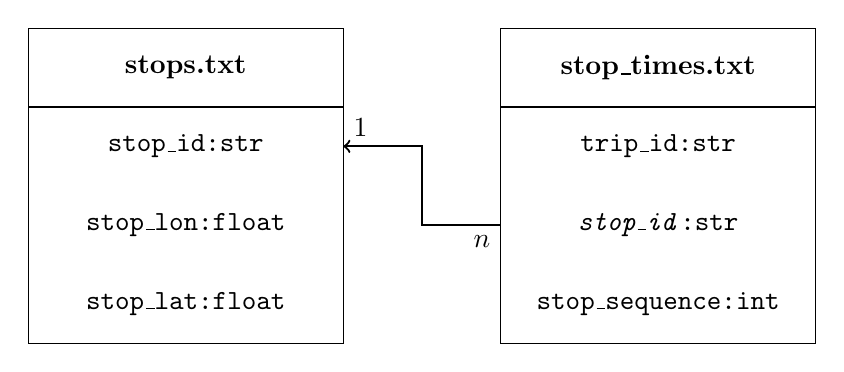
\begin{tikzpicture}
			\draw (0,3) rectangle +(4,1);
			\node at (2,3.5) {\bfseries stops.txt};
			\draw (0,0) rectangle +(4,4);
			\node at (2,2.5) {\ttfamily\bfseries stop\_id:str};
			\node at (2,1.5) {\ttfamily stop\_lon:float};
			\node at (2,.5) {\ttfamily stop\_lat:float};

			\draw (6,3) rectangle +(4,1);
			\node at (8,3.5) {\bfseries stop\_times.txt};
			\draw (6,0) rectangle +(4,4);
			\node at (8,2.5) {\ttfamily\bfseries trip\_id:str};
			\node at (8,1.5) {\ttfamily \textit{stop\_id}:str};
			\node at (8,.5) {\ttfamily stop\_sequence:int};

			\draw[thick,->] (6,1.5) node[anchor=north east] {\(n\)} -- ++(-1,0) -- ++(0,1) -- +(-1,0) node[anchor=south west] {\(1\)};
		\end{tikzpicture}
		\captionof{figure}{Database representation of the relevant GTFS files}
	\end{center}

	The nodes of the graph are directly given by the file \texttt{stops.txt}, so we can just parse the file to import them.
	This is done in the \texttt{import\_nodes} function of \hyperref[sec:code:gtfs]{\ttfamily gtfs.py} (line 40).

	Whereas the edges need some operations:
	\begin{enumerate}
		\item Parse the file
		\item Regroup in order the stops in the same trips
		\item Create edges between consecutive stops in a trip
	\end{enumerate}
	This is done in the \texttt{import\_edges} function of \hyperref[sec:code:gtfs]{\ttfamily gtfs.py} (line 56).

	\subsection{Creating a graph}\label{sec:step:1.2}

	The \texttt{Graph} class is in \hyperref[sec:code:graph]{\ttfamily graph.py}.

	The class supports weighted directed graphs, but unweighted or undirected graphs can also be created.\\
	The class constructor accepts an optional parameter which is a callback to compute weight from two given nodes.
	In our case, this function takes two \texttt{Stop} (\hyperref[sec:code:gtfs]{\ttfamily gtfs.py} line 8) instances and returns the Euclidian distance between them: \[
		\text{compute\_weight}: (s,s') \mapsto \sqrt{\left(s'_\text{lat} - s_\text{lat}\right)^2 + \left(s'_\text{lon} - s_\text{lon}\right)^2}
	\]
	If this parameter is not passed, all edge weights will be set to \(0\).\\
	The support for directions comes from the \texttt{neighbors\_in} and \texttt{neighbors\_out} methods.
	The method \texttt{neighbors} can be used instead for undirected graphs.

	\subsection{Results}\label{sec:results:1}

	\begin{itemize}
		\item \(7982\) lines from \texttt{stops.txt} were imported to \(7982\) nodes in the graph.
		\item \(1720661\) lines from \texttt{stop\_times.txt} were imported to \(8462\) edges in the graph.\\
		This is not surprising, because one line is used for a single stop in a single trip at certain hours: there are a lot of redundancies.
	\end{itemize}
	%TODO visual graph ?

	\section{Finding the shortest paths}\label{sec:step:2}

	%TODO

	\appendix
	\section{GTFS}\label{sec:code:gtfs}

	Main file, contains the code needed to import GTFS data to a graph.

	\lstinputlisting{src/gtfs.py}

	\section{Graph}\label{sec:code:graph}

	File that contains the \texttt{Graph} class.

	\lstinputlisting{src/graph.py}

	\section{Pathfinding (BFS \& Dijkstra)}\label{sec:code:pathfinding}

	File that contains the \texttt{bfs} and \texttt{dijkstra} functions.

	\lstinputlisting{src/pathfinding.py}
\end{document}
